\documentclass[11pt, notitlepage]{report}

	\usepackage[margin=1in]{geometry}
	\usepackage{amsmath,amsthm,amssymb,amsfonts}
	\usepackage{enumitem}
	\usepackage{systeme}

	\newcommand{\N}{\mathbb{N}}
	\newcommand{\Z}{\mathbb{Z}}
	\newcommand{\R}{\mathbb{R}}
	\newcommand{\A}{\alpha}
	\newcommand{\ora}[1]{\overrightarrow{#1}}
	\newcommand{\Question}[1]{\newpage\section{#1}}
	\usepackage[parfill]{parskip}
	\usepackage{mathtools}
	\newenvironment{solution}{\paragraph{\small Solution:}}{\hfill}
	\newenvironment{theorem}{\paragraph{Theorem:}}{\hfill}
	\newenvironment{definition}{\paragraph{Definition:}}{\hfill}
	\newenvironment{problem}[2][Problem]{\begin{trivlist}
	\item[\hskip \labelsep {\bfseries #1}\hskip \labelsep {\bfseries #2.}]}{\end{trivlist}}
	
	\usepackage{pgfplots}
	\usetikzlibrary{arrows}
	\usetikzlibrary{decorations.markings}
	\usetikzlibrary{datavisualization}
	\usetikzlibrary{datavisualization.formats.functions}
	%\usepackage{pstricks-add}

	\pgfplotsset{every axis/.append style={
	                   axis x line=middle,    % put the x axis in the middle
	                   axis y line=middle,    % put the y axis in the middle
	                   axis line style={<->,color=gray}, % arrows on the axis
	                   xlabel={$x$},          % default put x on x-axis
	                   ylabel={$y$},          % default put y on y-axis
	           }}
	\pgfplotsset{compat=1.15}
	
	\newcommand{\pgraph}[4]{
		\begin{center}
		
		\begin{tikzpicture}
		\begin{axis}[
		   trig format plots=rad,
		   axis equal,
		   grid=both
		]
		\addplot [domain=#3:#4, variable=\t, samples=50, black, decoration={
		   markings,
		   mark=between positions 0.2 and 1 step 4em with {\arrow [scale=1.5]{stealth}}
		   }, postaction=decorate]
		({#1}, {#2});
		
		\end{axis}
		\end{tikzpicture}
		
		\end{center}
	}


   \newcommand{\cgraph}[3]{
	   \begin{center}
	
	   \begin{tikzpicture}
	   \begin{axis}[
	       trig format plots=rad,
	       axis equal,
	       grid=both
	   ]
	   \addplot [domain=#2:#3, variable=\x, samples=50, black, decoration={
	       markings,
	       mark=between positions 0.2 and 1 step 4em with {\arrow [scale=1.5]{stealth}}
	       }, postaction=decorate]
	   {#1};
	
	   \end{axis}
	   \end{tikzpicture}
	
	   \end{center}
	}


	
	\makeatletter
	\newcommand*{\toccontents}{\@starttoc{toc}}
	\makeatother


\begin{document}
   \title{CS70: Homework 3}
   \author{Abhijay Bhatnagar}
   \maketitle
   \toccontents



\setcounter{secnumdepth}{0} %% no numbering

\section{Problem 1: Short Answer: Graphs}

\begin{enumerate}[label=(\alph*)]
\item
Bob removed a degree $3$ node in an $n$-vertex tree, how many connected
components are in the resulting graph?  (An expression that may
contain $n$.)

\item
Given an $n$-vertex tree, Bob added 10 edges to it, then Alice removed 
5 edges and the resulting graph has 3 connected components.
How many edges must be removed to remove all cycles
in the resulting graph? (An expression that may contain $n$.)

%\item
%Give a gray code for 3-bit strings. (Recall that a gray code is a
%sequence of bitstrings where adjacent elements differ by one.  For
%example, the gray code of 2-bit strings is $00,01,11,10$.  Note the
%last string is considered adjacent to the first and $10$ differs in
%one bit from $00$. Answer should be sequence of three-bit strings: 8
%in all.)

\item
True or False: For all $n \geq 3$, the complete graph on $n$ vertices, $K_n$ has more
edges than the $n$-dimensional hypercube. Justify your answer.


\item
A complete graph with $n$ vertices where $n$ is an odd prime can have all its edges
covered with $x$ Hamiltonian cycles (a Hamiltonian cycle is a cycle where
each vertex appears exactly once). What is the number, $x$,  of
such cycles required to cover the a complete graph? (Answer should be an expression that depends on $n$.)


\item
Give a set of edge-disjoint Hamiltonian cycles that covers the edges of $K_5$, the complete
graph on $5$ vertices.
(Each path should be a sequence (or list) of edges in $K_5$, where an edge is written as a pair of vertices from the set $\{0, 1, 2, 3, 4\}$ - e.g: $(0, 1), (1, 2)$.)


\end{enumerate}


\Question{Eulerian Tour and Eulerian Walk}

\begin{enumerate}[(a)]
    \item Is there an Eulerian tour in the graph above?

    \item Is there an Eulerian walk in the graph above?

    \item What is the condition that there is an Eulerian walk in an undirected graph? Briefly justfy your answer.
\end{enumerate}
\nosolspace{1cm}


\Question{Bipartite Graph}

A bipartite graph consists of $2$ disjoint sets of vertices (say $L$ and $R$), such that no $2$ vertices in the same set have an edge between them. 
% For example, if we had a bipartite graph that consists of vertices $\{1, 2, 3, 4\}$, such that set A = $\{1, 2\}$ and B = $\{3, 4\}$, there cannot exist an edge between $1$ and $2$, and similarly there cannot exist an edge between $3$ and $4$. \\
For example, here is a bipartite graph (with $L=\{\hbox{{\color{green}{green}} vertices}\}$ and $R =\{\hbox{{\color{red}{red}} vertices}\}$),  and a non-bipartite graph.

	\begin{figure}[hpb]
\begin{minipage}{0.49\textwidth}
	\centering
	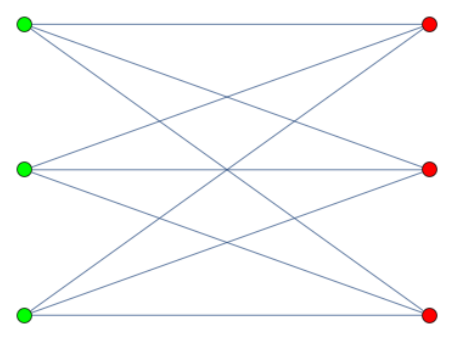
\includegraphics[scale=.3]{src/problems/graphtheory/resources/k_3_3.png}
\end{minipage}
\begin{minipage}{0.49\textwidth}
	\centering
	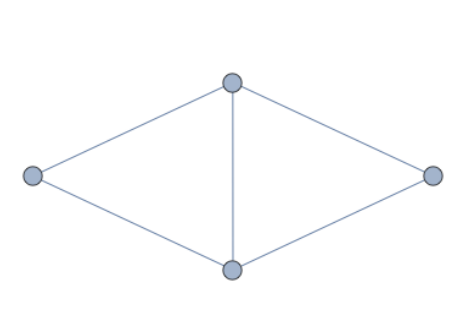
\includegraphics[scale=.3]{src/problems/graphtheory/resources/non-bipartite.png}
\end{minipage}
\caption{A bipartite graph (left) and a non-bipartite graph (right).}
	\label{fig:bipartite}
	\end{figure}

Prove that a graph is bipartite if and only if it has no tours of odd length.
\nosolspace{1in}


\Question{Hypercubes}

The vertex set of the $n$-dimensional hypercube $G=(V,E)$ is given by $V=\{0,1\}^n$ (recall that $\{0,1\}^n$ denotes the set of all $n$-bit strings). There is an edge between two vertices $x$ and $y$ if and only if $x$ and $y$ differ in exactly one bit position. These problems will help you understand hypercubes.

\begin{enumerate}
\item Draw 1-, 2-, and 3-dimensional hypercubes and label the vertices using the corresponding bit strings.

\nosolspace{1in}

% \item Show that the edges of an $n$-dimensional hypercube can be colored using $n$ colors so that no pair of edges sharing a common vertex have the same color.

% \nosolspace{1in}

%\item Show that the vertices of an $n$-dimensional hypercube can be colored using $2$ colors so that no pair of adjacent vertices have the same color. This is equivalent to showing that a hypercube is \emph{bipartite}: the vertices can be partitioned into two groups (according to color) so that every edge goes between the two groups.
\item Show that for any $n\ge 1$, the $n$-dimensional hypercube is \emph{bipartite}: the vertices can be partitioned into two groups so that every edge goes between the two groups.

\nosolspace{1in}

\end{enumerate}


\Question {Triangulated Planar Graph}
In this problem you will prove that every triangulated planar graph (every face has 3 sides; that is, every face has three edges bordering it, including the unbounded face)
contains either (1) a vertex of degree 1, 2, 3, 4, (2) two degree 5 vertices 
which are adjacent, or (3) a degree 5 and a degree 6 vertices which are 
adjacent. Justify your answers.

\begin{enumerate}
\item Place a ``charge'' on each vertex $v$ of value $6-\operatorname{degree}(v)$. What is
the sum of the charges on all the vertices?
(\textit{Hint}: Use Euler's formula and the fact that the planar graph is
triangulated.)


\item What is the charge of a degree $5$ vertex and of a degree $6$ vertex?


\item Suppose now that we shift $1/5$ of the charge of a degree $5$ vertex to each of its neighbors that has a negative charge.  (We refer to this as ``discharging'' the degree $5$ vertex.)  Conclude the proof under the assumption that, after discharging all degree $5$ vertices, there is a degree $5$ vertex with positive remaining charge.
%Move $1/5$ charge from each degree $5$ vertex to each of its negatively charged 
%neighbors. Conclude the proof in the case where there is a degree $5$
%vertex with positive remaining charge. 

\item If no degree $5$ vertices have positive charge after discharging the degree $5$ vertices, 
does there exist any vertex with positive charge after discharging?
If there is such a vertex, what are the possible degrees of that vertex?

\item 
Suppose there exists a degree $7$ vertex with positive charge after discharging the degree $5$ vertices.
How many neighbors of degree $5$ might it have?

\item Continuing from item (e). Since the graph is triangulated,
  are two of these degree $5$ vertices adjacent?

\item Finish the proof from the facts you obtained from the previous
  parts.



\end{enumerate}





\end{document}
